\rulechapter{Special Maneuvers}
\label{rule:special-maneuvers}

\x{
This chapter details specific flight actions used to change aircraft position and facing.

A maneuver is a distinct flight action. It may not be combined with turning, although turns and maneuvers can be performed in the same game turn. A maneuver may be started at any point in an aircraft's flight. Beginning a maneuver aborts a turn in progress and beginning a turn aborts a maneuver in progress. More than one maneuver may be performed in one game turn. Some maneuvers may restrict attacks and/or weapon launches.
}{
This rule describes slides, rolls, and other maneuvers aircraft can use to change their position and facing.

A maneuver is a distinct flight action. An aircraft may not simultaneously turn and maneuver, although it may do so separately in the same game turn. An aircraft can start a maneuver at any point in its flight. Beginning a maneuver aborts any turn in progress, and beginning a turn aborts a maneuver in progress. An aircraft may perform more than one maneuver in a game turn. Some maneuvers may restrict attacks, weapon launches, and radar use.

}

\changedin{2A}{2A-roll-preparatory-fps}{
\section{Preparatory HFPs}
}{
\section{Preparatory FPs}
}

% ISSUE: maneuver split between game turns?

\x{
A maneuver usually requires the expenditure of \changedin{2A}{2A-roll-preparatopry-fps}{HFPs}{FPs} in flight as preparatory moves prior to execution of the maneuver itself. \addedin{2B}{2B-maneuver-consecutive}{All of the preparatory FPs and the FP expended to execute the maneuver must be consecutive.} These “prep” moves actually represent the aircraft's forward movement while in the maneuver. An aircraft is considered to be performing a maneuver from the first expenditure of preparatory FPs until its actual execution. For Slide maneuvers, two preparatory HFPs are required and for most roll maneuvers \changedin{2A}{2A-roll-preparatopry-fps}{one preparatory HFP is}{preparatory FPs equal to {\onethird} of the aircraft's speed (rounded down) are} required. However, when performing \deletedin{2A}{2A-snap}{snap turns or any }maneuvers at high altitudes and speeds, additional penalty \changedin{2A}{2A-roll-preparatopry-fps}{HFPs}{FPs} must be expended prior to the maneuvers as follows:

\begin{itemize}
    \item In the HI band add +1 preparatory \changedin{2A}{2A-roll-preparatopry-fps}{HFP}{FP}.
    \item In the VH band add +2 preparatory \changedin{2A}{2A-roll-preparatopry-fps}{HFPs}{FPs}.
    \item In the EH band add +3 preparatory \changedin{2A}{2A-roll-preparatopry-fps}{HFPs}{FPs}.
    \item In the UH band add +4 preparatory \changedin{2A}{2A-roll-preparatopry-fps}{HFPs}{FPs}.
    \item At supersonic speeds, add +1 preparatory \changedin{2A}{2A-roll-preparatopry-fps}{HFP}{FP}.
\end{itemize}

Note: The speed \changedin{2A}{2A-roll-preparatopry-fps}{HFP}{FP} is used in addition to the others.
}{

Before executing certain maneuvers, an aircraft must expend preparatory FPs. These FPs represent the aircraft’s movement during the maneuver. The aircraft is performing the maneuver from the first preparatory FP until the FP expended to execute the maneuver. All of the preparatory FPs and the FP expended to execute the maneuver must be consecutive.

\paragraph{Preparatory FP Requirements.} Slide maneuvers normally require two preparatory HFPs, and displacement and lag roll maneuvers require preparatory FPs equal to {\onethird} of the aircraft’s speed (rounded down). However, maneuvers performed at altitude, at supersonic speeds, or by damaged aircraft require additional preparatory FPs, according to Table~\ref{table:preparatory-fps}.

%!TEX root = ../rules-working.tex
%LTeX: enabled=false

\begin{twocolumntablefloat}[t]
\begin{twocolumntable}

\tablecaption{table:preparatory-fps}{Preparatory FPs}
\begin{tabularx}{0.6\linewidth}{Lr}
\toprule
Slide&2 HFPs\\
Displacement Roll&{\onethird} of speed (round down)\\
Lag Roll&{\onethird} of speed (round down)\\
\midrule
\samewidth[l]{UH}{HI} altitude band (26--35)&$+1$\\
\samewidth[l]{UH}{VH} altitude band (36--45)&$+2$\\
\samewidth[l]{UH}{EH} altitude band (46--60)&$+3$\\
\samewidth[l]{UH}{UH} altitude band (61+)&$+4$\\
\midrule
Supersonic speeds&$+1$\\
\RAY[3A-LRR-roll-maneuvers]{Lag or displacement roll and LRR&$+1$}
Aircraft damage&Table~\ref{table:aircraft-damage-effects} or \ref{table:optional-damage}\\
\bottomrule
\end{tabularx}

\end{twocolumntable}
\end{twocolumntablefloat}


}

\addedin{2B}{2B-maneuver-carry}{
\paragraph{Carrying a Maneuver.} 

Sometimes a maneuver will not or cannot be completed in one game turn. In this case, the maneuver may be carried into the next game turn. The carried maneuver should be noted on the turn carry row of the aircraft log with:
\begin{itemize}

    \item the number of preparatory FPs expended for the maneuver so far,

    \item the maneuver type (SL, DR, LR, VR, or VS), and

    \item the direction (L or R).

\end{itemize}

For example, “2DRL” indicates the aircraft has expended 2 preparatory FPs on a displacement roll to the left.
}

\section{Slide Maneuvers}

% ISSUE: HFPs only for slides?

\silentlyaddedin{1C}{1C-figures}{
    \begin{onecolumnfigure}[p]
\centering
\begin{tikzfigure}{11.333\standardhexwidth}
\scriptsize

    \drawhexgrid{0}{0}{10}{4}

    \begin{athex}{1.00}{0.50}
        \drawdashedcounter  {+0.00}{+0.00}{90}
        \drawdashedcounter  {+0.00}{+1.00}{90}
        \drawaircraftcounter{+0.00}{+2.00}{90}{F-4}{}{}
        \drawaircraftcounter{+1.00}{+2.50}{90}{F-4}{}{}
        \drawdashedcounter  {+1.00}{+3.50}{90}
        \begin{scope}[shift={(135:0.3)},thick,->]
            \miniathex{0.00}{0.00}{\draw (90:0.1) -- (90:0.5);}
            \miniathex{0.00}{1.00}{\draw (90:0.1) -- (90:0.5);}
            \miniathex{1.00}{2.50}{\draw (90:0.1) -- (90:0.5);}
        \end{scope}
        \miniathex{+0.00}{+2.00}{\draw [thick,->] (30:0.35) -- (30:0.65);}
    \end{athex}


    \begin{athex}{2.50}{0.75}
        \drawdashedcounter{+0.00}{+0.00}{60}
        \drawdashedcounter{+0.50}{+0.75}{60}
        \drawaircraftcounter{+1.00}{+1.50}{60}{F-4}{}{}
        \drawaircraftcounter{+2.00}{+2.00}{60}{F-4}{}{}
        \drawdashedcounter{+2.50}{+2.75}{60}
        \begin{scope}[shift={(105:0.3)},thick,->]
            \miniathex{+0.00}{+0.00}{\draw (60:0.05) -- (60:0.4);}
            \miniathex{+0.50}{+0.75}{\draw (60:0.05) -- (60:0.4);}
            \miniathex{+2.00}{+2.00}{\draw (60:0.05) -- (60:0.4);}
        \end{scope}
        \miniathex{+1.00}{+1.50}{\draw [thick,->] (30:0.35) -- (30:0.65);}
    \end{athex}
    
    \begin{athex}{5.00}{0.50}
        \drawdashedcounter  {+0.00}{+0.00}{60}
        \drawdashedcounter  {+0.50}{+0.75}{60}
        \drawaircraftcounter{+1.00}{+1.50}{60}{F-4}{}{}
        \drawaircraftcounter{+2.00}{+2.00}{60}{F-4}{}{}
        \drawdashedcounter  {+2.50}{+2.75}{60}
        \begin{scope}[shift={(105:0.3)},thick,->]
            \miniathex{+0.00}{+0.00}{\draw (60:0.05) -- (60:0.4);}
            \miniathex{+0.50}{+0.75}{\draw (60:0.05) -- (60:0.4);}
            \miniathex{+2.00}{+2.00}{\draw (60:0.05) -- (60:0.4);}
        \end{scope}
        \miniathex{+1.00}{+1.50}{\draw [thick,->] (30:0.35) -- (30:0.65);}
        \begin{scope}[shift={(315:0.5)},anchor=west]
            \miniathex{+0.00}{+0.00}{\draw node {start position};}
            \miniathex{+0.50}{+0.75}{\draw node {preparatory HFP};}
            \miniathex{+1.00}{+1.50}{\draw node {preparatory HFP};}
            \miniathex{+2.00}{+2.00}{\draw node {slide execution};}
            \miniathex{+2.50}{+2.75}{\draw node {next HFP};}
        \end{scope}
    \end{athex}

    
\end{tikzfigure}

\x{
\figurecaption{figure:slide-maneuvers}{Slide Maneuvers}
}{
\figurecaption{figure:slide-maneuvers}{Slides to the right, each with two preparatory HFPs. The number of preparatory HFPs required depends on the aircraft speed and other factors. The execution of a slide is identical to that of a displacement roll, although other aspects are different.}
}

\end{onecolumnfigure}

    \begin{figure}[p]
\centering
\x{
\begin{tikzfigure}{1.0\linewidth}
\scriptsize

    \drawhexgrid[1]{11}{4.5}

    \begin{athex}{2.00}{0.00}
        \drawdashedcounter  {+0.00}{+1.00}{90}
        \drawaircraftcounter{+0.00}{+2.00}{90}{F-4}{}
        \drawaircraftcounter{+1.00}{+2.50}{90}{F-4}{}
        \drawdashedcounter  {+1.00}{+3.50}{90}
        \begin{scope}[shift={(135:0.3)},thick,->]
            \miniathex{0.00}{1.00}{\draw (90:0.1) -- (90:0.5);}
            \miniathex{1.00}{2.50}{\draw (90:0.1) -- (90:0.5);}
        \end{scope}
        \miniathex{+0.00}{+2.00}{\draw [thick,->] (30:0.35) -- (30:0.65);}
    \end{athex}

    \begin{athex}{3.50}{0.25}
        \drawdashedcounter{+0.50}{+0.75}{60}
        \drawaircraftcounter{+1.00}{+1.50}{60}{F-4}{}
        \drawaircraftcounter{+2.00}{+2.00}{60}{F-4}{}
        \drawdashedcounter{+2.50}{+2.75}{60}
        \begin{scope}[shift={(105:0.3)},thick,->]
            \miniathex{+0.50}{+0.75}{\draw (60:0.05) -- (60:0.4);}
            \miniathex{+2.00}{+2.00}{\draw (60:0.05) -- (60:0.4);}
        \end{scope}
        \miniathex{+1.00}{+1.50}{\draw [thick,->] (30:0.35) -- (30:0.65);}
    \end{athex}
    
    \begin{athex}{6.00}{0.00}
        \drawdashedcounter  {+0.50}{+0.75}{60}
        \drawaircraftcounter{+1.00}{+1.50}{60}{F-4}{}
        \drawaircraftcounter{+2.00}{+2.00}{60}{F-4}{}
        \drawdashedcounter  {+2.50}{+2.75}{60}
        \begin{scope}[shift={(105:0.3)},thick,->]
            \miniathex{+0.50}{+0.75}{\draw (60:0.05) -- (60:0.4);}
            \miniathex{+2.00}{+2.00}{\draw (60:0.05) -- (60:0.4);}
        \end{scope}
        \miniathex{+1.00}{+1.50}{\draw [thick,->] (30:0.35) -- (30:0.65);}
        \begin{scope}[shift={(315:0.5)},anchor=west]
            \miniathex{+0.50}{+0.75}{\draw node {start position};}
            \miniathex{+1.00}{+1.50}{\draw node {preparatory HFP};}
            \miniathex{+2.00}{+2.00}{\draw node {roll execution};}
            \miniathex{+2.50}{+2.75}{\draw node {next HFP};}
        \end{scope}
    \end{athex}

\end{tikzfigure}
\caption{Displacement Roll Maneuvers}
}{
\begin{tikzfigure}{1.0\linewidth}
\scriptsize

    \drawhexgrid[1]{11}{5.5}

    \begin{athex}{2.00}{1.00}
        \drawdashedcounter  {+0.00}{+0.00}{90}
        \drawdashedcounter  {+0.00}{+1.00}{90}
        \drawaircraftcounter{+0.00}{+2.00}{90}{F-4}{}
        \drawaircraftcounter{+1.00}{+2.50}{90}{F-4}{}
        \drawdashedcounter  {+1.00}{+3.50}{90}
        \begin{scope}[shift={(135:0.3)},thick,->]
            \miniathex{0.00}{0.00}{\draw (90:0.1) -- (90:0.5);}
            \miniathex{0.00}{1.00}{\draw (90:0.1) -- (90:0.5);}
            \miniathex{1.00}{2.50}{\draw (90:0.1) -- (90:0.5);}
        \end{scope}
        \miniathex{+0.00}{+2.00}{\draw [thick,->] (30:0.35) -- (30:0.65);}
    \end{athex}

    \begin{athex}{3.50}{1.25}
        \drawdashedcounter{+0.00}{+0.00}{60}
        \drawdashedcounter{+0.50}{+0.75}{60}
        \drawaircraftcounter{+1.00}{+1.50}{60}{F-4}{}
        \drawaircraftcounter{+2.00}{+2.00}{60}{F-4}{}
        \drawdashedcounter{+2.50}{+2.75}{60}
        \begin{scope}[shift={(105:0.3)},thick,->]
            \miniathex{+0.00}{+0.00}{\draw (60:0.05) -- (60:0.4);}
            \miniathex{+0.50}{+0.75}{\draw (60:0.05) -- (60:0.4);}
            \miniathex{+2.00}{+2.00}{\draw (60:0.05) -- (60:0.4);}
        \end{scope}
        \miniathex{+1.00}{+1.50}{\draw [thick,->] (30:0.35) -- (30:0.65);}
    \end{athex}
    
    \begin{athex}{6.00}{1.00}
        \drawdashedcounter  {+0.00}{+0.00}{60}
        \drawdashedcounter  {+0.50}{+0.75}{60}
        \drawaircraftcounter{+1.00}{+1.50}{60}{F-4}{}
        \drawaircraftcounter{+2.00}{+2.00}{60}{F-4}{}
        \drawdashedcounter  {+2.50}{+2.75}{60}
        \begin{scope}[shift={(105:0.3)},thick,->]
            \miniathex{+0.00}{+0.00}{\draw (60:0.05) -- (60:0.4);}
            \miniathex{+0.50}{+0.75}{\draw (60:0.05) -- (60:0.4);}
            \miniathex{+2.00}{+2.00}{\draw (60:0.05) -- (60:0.4);}
        \end{scope}
        \miniathex{+1.00}{+1.50}{\draw [thick,->] (30:0.35) -- (30:0.65);}
        \begin{scope}[shift={(315:0.5)},anchor=west]
            \miniathex{+0.00}{+0.00}{\draw node {start position};}
            \miniathex{+0.50}{+0.75}{\draw node {preparatory HFP};}
            \miniathex{+1.00}{+1.50}{\draw node {preparatory HFP};}
            \miniathex{+2.00}{+2.00}{\draw node {roll execution};}
            \miniathex{+2.50}{+2.75}{\draw node {next HFP};}
        \end{scope}
    \end{athex}
    
\end{tikzfigure}
\caption{Displacement rolls to the right, each with two preparatory HFPs. The number of preparatory HFPs required depends on the aircraft speed and other factors.}
}
\label{figure:displacement-roll-maneuvers}
\end{figure}

    
\x{
\begin{onecolumnfigure}[p]
\centering
\begin{fitwidth}{11.333\standardhexwidth}
\begin{tikzpicture}

\scriptsize

    \drawhexgrid{0}{0}{10}{3}

    \begin{athex}{1.00}{-0.50}
        \drawdashedcounter  {+0.00}{+1.00}{90}
        \drawaircraftcounter{+0.00}{+2.00}{90}{F-4}{}{}
        \drawaircraftcounter{+1.00}{+2.50}{120}{F-4}{}{}
        \drawdashedcounter  {+0.50}{+3.25}{120}
        \begin{scope}[shift={(135:0.3)},thick,->]
            \miniathex{0.00}{1.00}{\draw (90:0.1) -- (90:0.5);}
        \end{scope}
        \begin{scope}[shift={(165:0.3)},thick,->]
            \miniathex{1.00}{2.50}{\draw (120:0.05) -- (120:0.4);}
        \end{scope}
        \begin{scope}[shift={(30:0.2)}]
            \miniathex{+0.00}{+2.00}{\draw [thick,->] (0:0.25) -- (0:0.65);}
        \end{scope}
    \end{athex}

    \begin{athex}{2.50}{-0.25}
        \drawdashedcounter  {+0.50}{+0.75}{60}
        \drawaircraftcounter{+1.00}{+1.50}{60}{F-4}{}{}
        \drawaircraftcounter{+1.50}{+1.25}{90}{F-4}{}{}
        \drawdashedcounter  {+1.50}{+2.25}{90}
        \begin{scope}[shift={(105:0.3)},thick,->]
            \miniathex{+0.50}{+0.75}{\draw (60:0.05) -- (60:0.4);}
        \end{scope}
        \begin{scope}[shift={(45:0.3)},thick,->]
            \miniathex{+1.50}{+1.25}{\draw (90:0.1) -- (90:0.5);}
        \end{scope}
        \begin{scope}[shift={(255:0.4)}]
            \miniathex{+1.00}{+1.50}{\draw [thick,->] (0:0) -- (330:0.4);}
        \end{scope}
    \end{athex}
    
    \begin{athex}{5.00}{-0.50}
        \drawdashedcounter  {+0.50}{+0.75}{60}
        \drawaircraftcounter{+1.00}{+1.50}{60}{F-4}{}{}
        \drawaircraftcounter{+2.00}{+2.00}{90}{F-4}{}{}
        \drawdashedcounter  {+2.00}{+3.00}{90}
        \begin{scope}[shift={(105:0.3)},thick,->]
            \miniathex{+0.50}{+0.75}{\draw (60:0.05) -- (60:0.4);}
        \end{scope}
        \begin{scope}[shift={(135:0.3)},thick,->]
            \miniathex{+2.00}{+2.00}{\draw (90:0.1) -- (90:0.5);}
        \end{scope}
        \miniathex{+1.00}{+1.50}{\draw [thick,->] (30:0.35) -- (30:0.65);}
        \begin{scope}[shift={(315:0.5)},anchor=west]
            \miniathex{+0.50}{+0.75}{\draw node {start position};}
            \miniathex{+1.00}{+1.50}{\draw node {preparatory HFP};}
            \miniathex{+2.00}{+2.00}{\draw node {roll execution};}
            \miniathex{+2.00}{+3.00}{\draw node {next HFP};}
        \end{scope}
    \end{athex}
    
\end{tikzpicture}
\end{fitwidth}

\figurecaption{figure:lag-roll-maneuvers}{Lag Roll Maneuvers}
\end{onecolumnfigure}

}{

\begin{twocolumnfigure}

\begin{fitheight}{5.2\standardhexwidth}
\begin{tikzpicture}
    \setfiguresize{-2.6}{-2.6}{+2.6}{+2.6}
    \begin{scope}
        \drawevenhexgrid{-2}{-2}{5}{5}
        \drawdashedcounter{+0.00}{-2.00}{0}
        \drawdashedcounter{+0.00}{-1.00}{0}
        \drawaircraftcounter{+0.00}{+0.00}{90}{F-4}{}{}
        \drawaircraftcounter{+1.00}{+0.50}{120}{F-4}{}{}
        \drawdashedcounter{+0.50}{+1.25}{120}
        \begin{scope}[shift={(-0.25,+0.25)},thick,->]
            \miniathex{+0.00}{-2.00}{\draw (90:0.0) -- (90:0.45);}
            \miniathex{+0.00}{-1.00}{\draw (90:0.0) -- (90:0.45);}
        \end{scope}
        \begin{scope}[shift={(30:0.2)}]
            \miniathex{+0.00}{+0.00}{\draw [thick,->] (0:0.25) -- (0:0.65);}
        \end{scope}
        \begin{scope}[shift={((1.05,0.85))},thick,->]
            \miniathex{+0.00}{+0.00}{\draw [thick,->] (120:0.0) -- (120:0.45);}
        \end{scope}
    \end{scope}
\end{tikzpicture}
\end{fitheight}
\hfil
\begin{fitheight}{5.2\standardhexwidth}
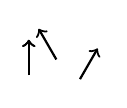
\begin{tikzpicture}
    \setfiguresize{-2.6}{-2.6}{+2.6}{+2.6}
    \begin{scope}[rotate=90]
        \drawevenhexgrid{-2}{-2}{5}{5}
        \drawdashedcounter{-2.00}{+0.00}{0}
        \drawdashedcounter{-1.00}{+0.00}{0}
        \drawaircraftcounter[90]{+0.00}{+0.00}{0}{F-4}{}{}
        \drawaircraftcounter[90]{+1.00}{-0.50}{30}{F-4}{}{}
        \drawdashedcounter{+2.00}{+0.00}{30}
        \begin{scope}[shift={(+0.20,+0.30)},thick,->]
            \miniathex{-2.00}{+0.00}{\draw (0:0.0) -- (0:0.45);}
            \miniathex{-1.00}{+0.00}{\draw (0:0.0) -- (0:0.45);}
        \end{scope}
        \begin{scope}[shift={(+0.40,-0.05)},thick,->]
            \miniathex{1.00}{-0.50}{\draw (30:0.0) -- (30:0.45);}
        \end{scope}
        \begin{scope}[shift={((0.15,-0.35))},thick,->]
            \miniathex{+0.00}{+0.00}{\draw [thick,->] (330:0.0) -- (330:0.45);}
        \end{scope}
        %\begin{scope}[shift={(0.0,+0.5)},anchor=east]
        %    \miniathex{-2.00}{+0.00}{\draw node {\minitable{r}{preparatory\\ HFP}};}
        %    \miniathex{-1.00}{+0.00}{\draw node {\minitable{r}{preparatory\\ HFP}};}
        %    \miniathex{+0.00}{+0.00}{\draw node {\minitable{r}{start\\ position}};}
        %    \miniathex{+1.00}{-0.50}{\draw node {\minitable{r}{roll\\ execution}};}
        %    \miniathex{+2.00}{+0.00}{\draw node {\minitable{r}{next\\ HFP}};}
        %\end{scope}
    \end{scope}
\end{tikzpicture}
\end{fitheight}
\hfil
\begin{fitheight}{5.2\standardhexwidth}
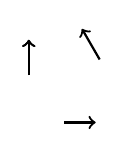
\begin{tikzpicture}
    \setfiguresize{-2.6}{-2.6}{+2.6}{+2.6}
    \begin{scope}[rotate=90]
        \drawoddhexgrid{-2}{-1.5}{5}{5}
        \drawdashedcounter{-2.00}{+0.00}{0}
        \drawdashedcounter{-1.00}{+0.00}{0}
        \drawaircraftcounter[90]{+0.00}{+0.00}{0}{F-4}{}{}
        \drawaircraftcounter[90]{+0.00}{-0.50}{30}{F-4}{}{}
        \drawdashedcounter{+1.00}{+0.00}{30}
        \begin{scope}[shift={(+0.20,+0.30)},thick,->]
            \miniathex{-2.00}{+0.00}{\draw (0:0.0) -- (0:0.45);}
            \miniathex{-1.00}{+0.00}{\draw (0:0.0) -- (0:0.45);}
        \end{scope}
        \begin{scope}[shift={(-0.40,-0.05)},thick,->]
            \miniathex{+0.00}{+0.00}{\draw (270:0.1) -- (270:0.5);}
        \end{scope}
        \begin{scope}[shift={(0.40,-0.60)},thick,->]
            \miniathex{+0.00}{+0.00}{\draw (30:0.0) -- (30:0.45);}
        \end{scope}
        \end{scope}
\end{tikzpicture}
\end{fitheight}


\figurecaption{figure:lag-roll-maneuvers}{Lag rolls to the right,each preceded by two preparatory HFPs and followed by another HFP. The execution of the roll is indicated by the counter images with solid borders. The number of preparatory FPs required depends on the aircraft speed and other factors.}

\end{twocolumnfigure}

}


}
\x{
A slide is an aircraft turn of less than 30 degrees. It requires a small angle of bank and (on the game map) no facing change. A sliding aircraft shifts one hex (or hexside) to the left or right without changing facing. \changedin{1C}{1C-figures}{The slide diagram}{Figure~\ref{figure:slide-maneuvers}} shows how it is executed.

\paragraph{Procedure.} Announce the start of a slide and its direction. Spend 2.0 or more in preparatory HFPs and spend 1.0 HFP to move the aircraft forward and to the left or right as announced.

\paragraph{Limits.} If the aircraft's start speed is 9.0 or less, it may perform one slide per game turn. If the start speed is greater than 9.0, two slides may be performed per game turn (an aircraft receives 1 decel point if it performs 2 slides in a game turn). If two slides are possible in the game turn, the aircraft must spend at least 4 FPs between the end of the first slide and the first preparatory HFP of the second slide.
}{
A slide is a turn of less than 30{\deg}. It requires a small angle of bank and (on the game map) produces a lateral displacement of one hex but no change of facing, as shown in Figure~\ref{figure:slide-maneuvers}.

\begin{itemize}
\item \itemparagraph{SL Requirements.} If an aircraft's start speed is 9.0 or less, it may perform one slide per game turn. If its start speed is 9.5 or greater, it may perform two slides per game turn but must additionally use at least 4 FPs between the end of the first slide and the first preparatory HFP of the second.

\item \itemparagraph{SL Procedure.} Declare the start of a slide and its direction. Use 2 or more preparatory HFPs, plus any additional HFPs from Table~\ref{table:preparatory-fps}, and then 1 HFP to execute the slide and move the aircraft forward and to the left or right as declared, as shown in Figure~\ref{figure:slide-maneuvers}.

\item \itemparagraph{SL DPs.} If an aircraft only performs one slide in a game turn, it receives no DPs. If it performs two, it receives 1 DP.

\end{itemize}

}
\section{Rolling Maneuvers}
\label{rule:rolling-maneuvers}

Rolling maneuvers use the outcome of a roll to change position and possibly facing.

\subsection{Displacement Rolls}

\x{
A displacement roll is a rapid snap-roll that allows an aircraft to shift left or right exactly as in a slide.
}{
A displacement roll (DR) is a rapid snap-roll that allows an aircraft to shift left or right exactly as in a slide.
}

\x{
\begin{itemize}
    \item\itemparagraph{DR Procedure.} Announce the start of a displacement roll and its direction. Spend \changedin{2A}{2A-roll-preparatopry-fps}{1.0 or more in preparatory FPs}{preparatory FPs equal to {\onethird} of the aircraft's speed (rounded down), plus additional FPs because of speed or altitude,} and spend 1.0 HFPs to execute the displacement roll, shift the aircraft forward and to the left or right as announced.\addedin{2A}{2A-roll-preparatopry-fps}{ The preparatory FPs may be HFPs or VFPs, but the FP used to execute the roll must be an HFP.}  The aircraft receives decel points as shown on the ADC. \changedin{1C}{1C-figures}{The displacement roll diagram}{Figure~\ref{figure:displacement-roll-maneuvers}} shows the resulting position shift.

\end{itemize}
}{
\paragraph{DR Procedure.} Declare the start of a displacement roll and its direction. Expend preparatory VFPs or HFPs equal to {\onethird} of the aircraft's speed (rounded down), plus additional VFPs or HFPs from Table~\ref{table:preparatory-fps}, and then spend 1 HFP to execute the displacement roll and move the aircraft forward and to the left or right as declared, as shown in Figure~\ref{figure:displacement-roll-maneuvers}.

\paragraph{DR DPs.} The aircraft receives DPs according to the ADC. For the second or subsequent displacement, lag, or vertical roll maneuver in a game turn, it receives one additional DP.
}

\subsection{Lag Rolls}

\x{
A lag roll is a modified displacement roll in which the pilot uses a combination of rudder and pitch control to pull the aircraft's nose to the inside of the roll effecting a facing change in the direction opposite the roll.
}{
A lag roll (LR) is a modified displacement roll in which the pilot uses a combination of rudder and pitch control to pull the aircraft's nose to the inside of the roll effecting a facing change in the direction opposite the roll.
}

\x{
\begin{itemize}
    \item\itemparagraph{LR Procedure.} Announce the start of a lag roll and its direction. Spend \changedin{2A}{2A-roll-preparatopry-fps}{1.0 or more in preparatory FPs}{preparatory FPs equal to {\onethird} of the aircraft's speed (rounded down), plus additional FPs because of speed or altitude,} and spend 1.0 in HFPs to execute the lag roll. Shift the aircraft forward and to the left or right as announced then change the facing by 30 degrees as depicted in  \changedin{1C}{1C-figures}{the lag roll diagram}{Figure~\ref{figure:lag-roll-maneuvers}}.\addedin{2A}{2A-roll-preparatopry-fps}{ The preparatory FPs may be HFPs or VFPs, but the FP used to execute the roll must be an HFP.} The aircraft receives decel points as shown on the ADC.
\end{itemize}
}{
\paragraph{LR Procedure.} Declare the start of a lag roll and its direction. Expend preparatory VFPs or HFPs equal to {\onethird} of the aircraft's speed (rounded down), plus additional VFPs or HFPs from Table~\ref{table:preparatory-fps}, and then spend 1 HFP to execute the displacement roll and move the aircraft forward and to the left or right as declared, as shown in Figure~\ref{figure:lag-roll-maneuvers}.

\paragraph{LR DPs.} The aircraft receives DPs according to the ADC. For the second or subsequent displacement, lag, or vertical roll maneuver in a game turn, it receives one additional DP.
}

\subsection{Barrel Rolls}

\silentlyaddedin{1C}{1C-figures}{
    \begin{onecolumnfigure}[tbp]
\CX{
\begin{fitwidth}{7.333\standardhexwidth}
\begin{tikzpicture}

\scriptsize

    \drawhexgrid{0}{0}{6}{5}

    \begin{athex}{0.00}{0.00}
        \drawdashedcounter  {+0.50}{+0.75}{60}
        \drawaircraftcounter{+1.00}{+1.50}{60}{F-4}{}{}
        \drawaircraftcounter{+2.00}{+2.00}{90}{F-4}{}{}
        \begin{scope}[shift={(105:0.3)},thick,->]
            \miniathex{+0.50}{+0.75}{\draw (60:0.05) -- (60:0.4);}
        \end{scope}
        \miniathex{+1.00}{+1.50}{\draw [thick,->] (30:0.35) -- (30:0.65);}
        \begin{scope}[shift={(315:0.5)},anchor=west]
            \miniathex{+0.50}{+0.75}{\draw node {start position};}
            \miniathex{+1.00}{+1.50}{\draw node {preparatory HFP};}
            \miniathex{+2.00}{+2.00}{\draw node {first roll execution};}
            \miniathex{+2.00}{+3.00}{\draw node {preparatory HFP};}
            \miniathex{+3.00}{+3.50}{\draw node {second roll execution};}
            \miniathex{+3.00}{+4.25}{\draw node {preparatory HFP};}
            \miniathex{+3.00}{+5.00}{\draw node {third roll execution};}
        \end{scope}
        \begin{scope}[shift={(345:0.5)},anchor=west]
        \end{scope}
    \end{athex}

    \begin{athex}{2.00}{1.00}
        \drawaircraftcounter{+0.00}{+2.00}{90}{F-4}{}{}
        \drawaircraftcounter{+1.00}{+2.50}{120}{F-4}{}{}
        \begin{scope}[shift={(135:0.3)},thick,->]
            \miniathex{0.00}{1.00}{\draw (90:0.1) -- (90:0.5);}
        \end{scope}
        \begin{scope}[shift={(30:0.2)}]
            \miniathex{+0.00}{+2.00}{\draw [thick,->] (0:0.25) -- (0:0.65);}
        \end{scope}
    \end{athex}

    \begin{athex}{3.50}{2.75}
        \drawaircraftcounter{-1.00}{+1.50}{120}{F-4}{}{}
        \drawaircraftcounter{-0.50}{+1.75}{150}{F-4}{}{}
        \begin{scope}[shift={(165:0.3)},thick,->]
            \miniathex{-0.50}{+0.75}{\draw (120:0.05) -- (120:0.4);}
        \end{scope}
        \begin{scope}[shift={(315:0.4)},thick,->]
            \miniathex{-1.00}{+1.50}{\draw (30:0.1) -- (30:0.5);}
        \end{scope}
    \end{athex}
    
\end{tikzpicture}
\end{fitwidth}

\figurecaption{figure:barrel-roll-maneuvers}{Barrel Roll Maneuvers.}

}{
\begin{fitheight}{9.2\standardhexwidth}
\begin{tikzpicture}
\scriptsize

    \setfiguresize{-2.6}{-4.6}{+6.1}{+4.6}
    \drawevenhexgrid{-2}{-4}{9}{9}

    \begin{athex}{-1.00}{-3.50}
        \drawdashedcounter  {+0.00}{+0.00}{60}
        \drawdashedcounter  {+0.50}{+0.75}{60}
        \drawaircraftcounter{+1.00}{+1.50}{60}{F-4}{}{}
        \drawaircraftcounter{+2.00}{+2.00}{90}{F-4}{}{}
        \begin{scope}[shift={(105:0.3)},thick,->]
            \miniathex{+0.50}{+0.75}{\draw (60:0.05) -- (60:0.4);}
        \end{scope}
        \begin{scope}[shift={(135:0.3)},thick,->]
            \miniathex{+2.00}{+2.00}{\draw (90:0.1) -- (90:0.5);}
        \end{scope}
        \miniathex{+1.00}{+1.50}{\draw [thick,->] (30:0.35) -- (30:0.65);}
        \begin{scope}[shift={(315:0.5)},anchor=west]
            \miniathex{+0.00}{+0.00}{\draw node {start position};}
            \miniathex{+0.50}{+0.75}{\draw node {preparatory HFP};}
            \miniathex{+1.00}{+1.50}{\draw node {preparatory HFP};}
            \miniathex{+2.00}{+2.00}{\draw node {first roll execution};}
            \miniathex{+2.00}{+3.00}{\draw node {preparatory HFP};}
            \miniathex{+2.00}{+4.00}{\draw node {preparatory HFP};}
            \miniathex{+3.00}{+4.50}{\draw node {second roll execution};}
        \end{scope}
        \begin{scope}[shift={(345:0.5)},anchor=west]
            \miniathex{+2.50}{+5.25}{\draw node {preparatory HFP};}
            \miniathex{+2.00}{+6.00}{\draw node {preparatory HFP};}
            \miniathex{+2.00}{+7.00}{\draw node {third roll execution};}
        \end{scope}
    \end{athex}
    
    \begin{athex}{1.00}{-1.50}
        \drawdashedcounter  {+0.00}{+1.00}{90}
        \drawaircraftcounter{+0.00}{+2.00}{90}{F-4}{}{}
        \drawaircraftcounter{+1.00}{+2.50}{120}{F-4}{}{}
        \begin{scope}[shift={(135:0.3)},thick,->]
            \miniathex{0.00}{1.00}{\draw (90:0.1) -- (90:0.5);}
        \end{scope}
        \begin{scope}[shift={(165:0.3)},thick,->]
            \miniathex{1.00}{2.50}{\draw (120:0.05) -- (120:0.4);}
        \end{scope}
        \begin{scope}[shift={(30:0.2)}]
            \miniathex{+0.00}{+2.00}{\draw [thick,->] (0:0.25) -- (0:0.65);}
        \end{scope}
    \end{athex}

    \begin{athex}{2.00}{1.00}
        \drawdashedcounter  {-0.50}{+0.75}{120}
        \drawaircraftcounter{-1.00}{+1.50}{120}{F-4}{}{}
        \drawaircraftcounter{-1.00}{+2.50}{120}{F-4}{}{}
        \begin{scope}[shift={(165:0.3)},thick,->]
            \miniathex{-0.50}{+0.75}{\draw (120:0.05) -- (120:0.4);}
        \end{scope}
        \begin{scope}[shift={(45:0.3)},thick,->]
            \miniathex{-1.00}{+1.50}{\draw (90:0.1) -- (90:0.5);}
        \end{scope}
    \end{athex}

\end{tikzpicture}
\end{fitheight}

\figurecaption{figure:barrel-roll-maneuvers}{A barrel roll executed as a sequence of two lag rolls to the right followed by one displacement roll to the right, each with two preparatory HFPs. Any combination of lag rolls and displacement rolls may make up a barrel roll, but all must be in the same direction. The number of preparatory FPs required before each roll depends on the aircraft speed and other factors.}
}

\end{onecolumnfigure}

}

\x{
A barrel roll is a large version of a lag roll or displacement roll. The barrel roll is performed gamewise as a series of two or more connected lag or displacement rolls in the same direction (in actual flight, the pilot would be doing one big roll instead of several small ones).

Multiple lag rolls or displacement rolls in the same game turn, but with FPs expended between one roll and the preparatory move of the next, or rolls done in opposite directions, are not a considered a barrel roll.
}{
A barrel roll (BR) is a larger version of a lag roll or displacement roll. In the game, it is performed as a series of two or more consecutive lag or displacement rolls in the same direction. In actual flight, the pilot would execute one longer and larger roll instead of several small ones. Figure~\ref{figure:barrel-roll-maneuvers} shows the resulting position shifts of a barrel roll done as two lag rolls and one displacement roll performed consecutively.

Multiple lag or displacement rolls that are not consecutive or that are consecutive but are not in the same sense are not considered to be a barrel roll.
}

\x{
\begin{itemize}
    \item\itemparagraph{BR Procedure.} Announce the start of a barrel roll and execute it as a series of two or more lag rolls and/or displacement rolls. \changedin{1C}{1C-figures}{The barrel roll diagram}{Figure~\ref{figure:barrel-roll-maneuvers}} shows the resulting position shifts of a barrel roll done as three connected lag rolls.
\end{itemize}
}{
\paragraph{BR Procedure.} Declare the start of a barrel roll and execute it as a series of two or more lag or displacement rolls.

\paragraph{BR DPs.} The aircraft receives DPs normally for each displacement or lag roll in the barrel roll.

}

\deletedin{1C}{1C-figures}{Note: All of the Maneuver Diagrams are in the play aids.}

\subsection{Vertical Rolls}

\x{
When flying straight up or down, an aircraft can easily roll about its longitudinal axis changing facing in the process. In reality, facing has no meaning going straight up or down but upon recovery from a vertical climb or dive any amount of roll would manifest itself as a heading change.
}{
In vertical flight, aircraft can roll easily. Such a vertical roll (VR) results in a change in direction after recovery from the climb or dive into horizontal flight.
}

\x{
\begin{itemize}

    \item\itemparagraph{VR Limits.} A vertical roll may only be performed by an aircraft in a vertical climb or vertical dive. It may only be performed from a hex or hexside in which the aircraft just expended a VFP. Multiple vertical rolls are allowed in a game turn, but only once per VFP expended.

    \item\itemparagraph{VR Procedure.} Announce the vertical roll and its direction at the moment of execution. No prep move is required. There is no FP cost. The ADC indicates any Decel point cost for a Vertical Roll. The aircraft may change facing \deletedin{1E}{AWF}{up} by 30 degrees up to 6 times in the chosen direction for each VR executed. If on a hexside, and it faces less than 6 times, the aircraft must shift left or right (as for a turn); otherwise it may stay on the line or shift as desired during the roll.  Incur 1 extra Decel for every vertical roll beyond the first in a game-turn in addition to normal roll costs.

\end{itemize}

\paragraph{Low Roll Rate Restriction.} A low Roll Rate aircraft is limited to three 30{deg} facing changes per Vertical roll executed.

\paragraph{High Pitch Rate Restriction.} If a High Pitch Rate aircraft uses its HPR ability to enter a vertical climb from level flight, then it may only do a vertical roll at the end of its flight, and only if the last FP expended was a VFP.
}{

\paragraph{VR Requirements.} A vertical roll may only be performed by an aircraft in a vertical climb or vertical dive (see rule\ref{rule:vertical-climbs} and \ref{rule:vertical-dives}). It may only be performed when the aircraft has just expended a VFP. Multiple vertical rolls are allowed in a game turn, but only one per VFP expended.

\paragraph{VR Procedure.} Declare the vertical roll and its direction at the moment of execution. No preparatory FPs are required. Expend 1 VFP to execute the roll and change facing by 30{\deg} up to 6 times in the chosen direction. 

If an aircraft executes a vertical roll on a hex side and it changes facing by less than 180{\deg}, it must shift to the adjacent hex in the sense of the roll. Otherwise, it may stay on the hex side or shift to the adjacent hex as desired.

\paragraph{VR DPs.} The aircraft receives DPs according to the ADC. For the second or subsequent displacement, lag, or vertical roll maneuver in a game turn, it receives one additional DP.

\paragraph{Low Roll Rate Restriction.} If an ADC notes that an aircraft has a
a low roll rate (LRR), it is limited to three 30{\deg} facing changes per vertical roll executed.

\paragraph{High Pitch Rate Restriction.} If an ADC notes that an aircraft has a high pitch rate (HPR) and it uses this capacity to enter a vertical climb from level flight (see rule\ref{rule:vertical-climbs}), then it may only perform a vertical roll at the end of its flight and only if the last FP expended is a VFP.
}
\subsection{Half-Rolls and Dives}
\label{rule:half-rolls-and-dives}

\x{
Aircraft often invert in order to enter dives quickly as they have better positive G pitch rates than negative G ones; meaning, it is easier to pull toward the top of the aircraft than push toward the bottom. 
}{
To enter a dive quickly, an aircraft can use a half-roll and dive (HRD) maneuver, in which it rolls inverted, then pitches positively, and finally rolls upright again. This maneuver is often quicker than simply pitching negatively since positive pitch rates are often better than negative ones.
}

\x{
An aircraft that executes a half-roll and dive may do one of the following:

\begin{itemize}

    \item Immediately enter a vertical dive from level flight.

    \item Enter a vertical dive from a zoom or sustained climb if its start speed is 4.0 or less.

    \item Enter a steep dive from a vertical climb.

\end{itemize}

Note: Use of the half-roll and dive avoids the restrictions against diving flight imposed by vertically climbing, and avoids the restrictions against entering vertical dives without previously using diving flight.    
}{

A half-roll and dive allows an aircraft to avoid the normal requirement of diving flight before a vertical dive (see rule~\ref{rule:vertical-dives}) and the normal prohibition of diving flight after a vertical climb (see rule~\ref{rule:vertical-climbs}). Specifically, an aircraft that executes a half-roll and dive may:

\begin{itemize}

    \item Enter a vertical dive directly from level flight.

    \item Enter a vertical dive directly from a zoom or sustained climb, provided its speed is 4.0 or less.

    \item Enter a steep dive directly from a vertical climb.

\end{itemize}

\paragraph{HRD Requirements.} The aircraft must have used level or climbing flight in the previous game turn. If it used a zoom or sustained climb, its speed must be 4.0 or less.

\paragraph{HRD Procedure.} At the beginning of the aircraft's flight, declare a half-roll and dive and the appropriate diving flight type according to the flight type used in the previous game turn: a steep dive after a vertical climb and a vertical dive otherwise. A half-roll and dive requires no preparatory FPs and does not require an FP to execute.

\paragraph{HRD DPs.} An aircraft does not receive DPs for executing a half-roll and dive.
    
%Announce the half-roll and dive at the beginning of the aircraft's flight. The aircraft immediately inverts at no cost (in FPs or decel points) and may now conduct normal diving flight, Steep or Vertical dive as appropriate. The aircraft is considered upright (not inverted) again at the end of its flight.
}

\x{
\paragraph{Restrictions.} A half-roll and dive restricts aircraft as follows:

\begin{itemize}

    \itemaddedin{1B}{1B-apj-36-errata}{When this maneuver is used to go from level flight to a vertical dive the first FP must be an HFP.}

    \itemaddedin{1B}{1B-apj-23-qa and 1B-apj-23-errata}{When this maneuver is used to go from a zoom or sustained climb to a vertical dive, the restrictions of 5.5 would apply in that all of the available HFPs (1/3 of the FPs) must be used before any VFPs are whether the aircraft is a high pitch rate or not. When used to go from a vertical climb directly to a steep dive, rule 5.5 applies in full. HPR aircraft must expend 1/3d their FPs as HFPs first and others 1/2. An aircraft going from a vertical climb to a steep dive this way may do normal turning but may not do any other maneuvers in that turn.}

    \item No other maneuvers are permitted except for one final vertical roll allowed at the end of the aircraft's flight if the last FP was a VFP.

    \item No attacks, weapon launches, or radar work (except boresight, auto-track) are permitted in the game-turn.
    
\end{itemize}
}{
\paragraph{HRD Restrictions.} An aircraft executing a half-roll and dive is restricted as follows:

\begin{itemize}

    \item When an HRD is used to enter a vertical dive from level flight, advanced rule~\ref{rule:changing-flight-type} applies, and the first FP must be an HFP.

    \item When a HRD is used to enter a vertical dive from a zoom or sustained climb, all of the available HFPs (that is, 1/3 of the FPs) must be used before any VFPs is used, regardless of whether the aircraft is noted as having a high pitch rate or not. This restriction supersedes advanced rule~\ref{rule:changing-flight-type} on the transition from climbing to diving flight,
    
    \item When an HRD is used to enter a steep dive from a vertical climb, advanced rule~\ref{rule:changing-flight-type} applies, and a normal aircraft must expend 1/2 of its FPs as HFPs before expending any VFPs. If an aircraft's ADC notes that it has a high pitch rate, it must expend only 1/3 of its FPs as HFPs before expending any VFPs.
    
    \item When an HRD is used to enter a steep dive, an aircraft may turn normally, but no other maneuvers are permitted during the game turn.

    \item When an HRD is used to enter a vertical dive, only one vertical roll is permitted during the game turn, and this can only be after the last FP, provided this FP is a VFP.

    \item No attacks, weapon launches, or radar work (except using boresight or auto-track modes) are permitted in the game turn.
    
\end{itemize}

}
\label{rule:sustained-rolling-maneuvers}

\x{
\subsection{Penalties and Restrictions on Rolling Maneuvers}

All rolling maneuvers produce the following penalties and restrictions on aircraft:

\paragraph{Additional Decel Points.} In any game turn in which more than one roll maneuver was performed, extra decel points are incurred. For each lag, displacement, and/or vertical roll performed after the first, an aircraft receives 1.0 decel points in addition to normal roll costs.

Each lag roll or displacement roll in a barrel roll is counted as an individual roll. Even rolls which normally produce 0 Decel points are counted for this penalty.

\paragraph{Weapons Restrictions.} Guns may not be fired, nor weapons launched, if the FP expended immediately prior to those desired actions was used to prepare for or execute a roll of any type.

\paragraph{Radar Tracking.} Radar lock-ons held by the aircraft against other aircraft are lost the moment it does any rolling maneuver other than a vertical roll. The lock-on is also lost if more than one vertical roll is done in a game turn.

\paragraph{Turn Rates.} For purposes of gunsight tracking, or missile launch G modifiers, a roll maneuver counts as turning at the BT turn rate.

\paragraph{High Altitude Maneuvering Departures.} An aircraft attempting rolling maneuvers in the EH altitude or UH bands risks a maneuvering departure. Upon executing any roll at EH or higher, roll one die. On a result of 4 or less, the aircraft suffers a maneuvering departure.
}{
\subsection{Additional Penalties and Restrictions}

Aircraft executing rolling maneuvers suffer the following penalties and restrictions:

\paragraph{Additional DPs.} 
For the second or subsequent lag, displacement, or vertical roll executed in a game turn, an aircraft receives 1 additional DP beyond the DPs noted in the ADC. Even rolls for which an aircraft normally receives 0 DPs are counted for this penalty. For these purposes, each lag roll or displacement roll in a barrel roll is counted as one roll.

For example, if an aircraft executed a lag, displacement, and vertical roll in a game turn, it would receive 2 DPs beyond those noted in the ADC.

\paragraph{Weapons Restrictions.} An aircraft may not attack with guns or rockets or launch weapons immediately after an FP used to prepare for or execute a rolling maneuver.

\paragraph{Turn Rate Modifiers.} During the recovery period after a rolling maneuver (see rule~\ref{rule:recovery-periods}), an aircraft suffers gun and rocket attack modifiers and missile launch G modifiers as if it were recovering from a turn at the BT rate.

\paragraph{Radar Tracking.} Radar lock-ons held by the aircraft are lost when it uses an FP to prepare for or execute a displacement, lag, or barrel roll, declares a half-roll and dive, or executes more than one vertical roll in a game turn.

\paragraph{High-Altitude Maneuvering Departures.} An aircraft attempting a rolling maneuver in the EH or UH altitude bands risks a maneuvering departure (see advanced rule~\ref{rule:maneuvering-departures}). Upon executing any roll in these altitude bands,  roll one die. On a result of $4-$, the aircraft suffers a maneuvering departure.
}

\begin{advancedrules}

\section{Climbing and Diving Barrel Rolls}

An aircraft may change altitude while barrel rolling if it is also in climbing or diving flight (and to a limited degree if in level flight).

When an aircraft executes a climbing or diving barrel roll, it may gain or lose one level of altitude respectively for each lag or displacement roll \changedin{1B}{1B-apj-30-qa}{component of}{executed as part of} the barrel roll after the first. There is no additional cost in FPs for this altitude gain or loss.

The barrel roll altitude change may be done in place of, or in conjunction with, VFPs expended for normal climbing and diving and satisfies the requirement for choosing a specific climb and dive type. For purposes of nose attitude, a climbing or diving barrel roll is considered a zoom climb or steep dive respectively.

\addedin{1B}{1B-apj-36-errata}{An aircraft choosing to barrel roll in climbing flight is in a zoom climb, except that it need not expend any VFPs, all FPs could be HFPs. Aircraft can perform diving barrel rolls if either steep or unloaded dives are performed, except that no steep dive VFPs need to actually be expended as long as altitude loss requirements are met by the diving rolls.}

\paragraph{Limited Climbing Or Diving Barrel Roll.} When a barrel roll ls executed from level flight, only one level may be gained or lost and only upon executing the last roll in the entire maneuver.

\paragraph{Decel Points.} An aircraft which changes altitude in a barrel roll receives 2.0 decel points per altitude level gained, and 0.5 accel points per altitude level lost.

\x{
\section{Vertical Reverse Maneuver}
}{
\section{Vertical Reverse Maneuvers}
}
\label{rule:vertical-reverses}

\x{
A vertical reverse (sometimes called a hammer-head stall or pitch-over) is a maneuver in which an aircraft enters a vertical climb and just prior to stalling, the pilot kicks the rudder and coordinates the controls to cause the aircraft to reverse its direction in the stall. It is difficult to perform.

\paragraph{Procedure.} An aircraft in a vertical climb may, if it ends its move at or no more than 1.0 below minimum speed, attempt a vertical reverse in the next stalled aircraft phase,

\paragraph{Announce Vertical Reverse in the Stalled Aircraft Phase.} Roll for stall/departure normally even if at minimum speed. If the aircraft departs, it must do departed flight. If it does not depart, it rolls again immediately to see if it successfully reverses. The roll required to vertical reverse is the same as the roll for recovering from a departure. (The same modifiers apply as well). 

If successful, the aircraft enters a vertical dive and is exempted from the requirement to first spend HFPs (when switching between climbs and dives). The aircraft's start speed is changed to its minimum speed (lose any \changedin{1E}{AWF}{.5}{0.5} carry if it started below minimum speed). It moves in normal order and may affect order of flight. If unsuccessful, it enters stalled flight.
}{
A vertical reverse (sometimes called a hammer-head stall or pitch-over) is a maneuver in which an aircraft enters a vertical climb and just prior to stalling, the pilot kicks the rudder and coordinates the controls to cause the aircraft to reverse its direction in the stall. It is difficult to perform.

\paragraph{VR Requirements.} The aircraft must have used a vertical climb in the previous game turn and have a speed no more its minimum speed and no less than its minimum speed minus 1.0 (i.e., its speed must be minimum speed, minimum speed minus 0.5, and minimum speed minus 1.0).

\paragraph{VR Procedure.} Announce the vertical reversal in the stalled aircraft phase. 

\begin{itemize}

\item Check for avoiding departed flight (see rule~\ref{rule:abnormal-flight}), even if the aircraft is at its minimum speed. If unsuccessful, it enters departed flight. 

\item If it does not depart, roll again immediately to see if it successfully reverses. The roll required for success is the same as that required to recover from departured flight and the same modifiers apply. If unsuccessful, it enters stalled flight.

\item If successful, the aircraft enters a vertical dive and is exempted from the requirement to first expend HFPs when switching between climbing and diving flight (see advanced rule~\ref{rule:changing-flight-type}). The aircraft's speed is immediately changed to its minimum speed and it loses any 0.5 FP it may have carried in. It then moves normally and may affect the order of flight.

\end{itemize}

\paragraph{VR DPs.} An aircraft does not receive DPs for executing a vertical reverse.

}

\section{VIFF Maneuvers}
\label{rule:viff-maneuvers}

Vectoring in forward flight (VIFF) is the ability of an aircraft to use movable thrust nozzles and/or special control surfaces to maneuver in directions normally impossible with traditional control surfaces. An aircraft noted as being VIFF capable can perform VIFF maneuvers. \addedin{1B}{1B-apj-23-errata}{VIFF maneuvers require Mil or AB power settings.}

\subsection{VIFF Sidestep}

The aircraft executes a slide maneuver, but pays different costs for the result.

\paragraph{Procedure.} During flight, announce the start of a VIFF sidestep and its direction. The aircraft spends no HFPs in preparation at MH or lower (it spends 1 HFP in preparation at HI or VH; it spends 2 HFPs in preparation at EH and UH). To execute the VIFF sidestep, the aircraft pays 2 HFPs and receives 2 decel points.

More than one VIFF sidestep may be performed in a game turn, but the aircraft must spend at least one HFP between each sidestep (turning in the direction of the sidestep is allowed during this HFP). The aircraft must reverse its angle of bank if it sidesteps one way and then desires to sidestep the other way.

\subsection{VIFF Assisted Turning}

Vectored thrust is used to aid a turn. Turn the aircraft normally but reduce the listed FP requirement by one for any given turn rate. If the FP requirement is already 1, then use 60{deg}. If it is already 60{deg} or 90{deg}, a VIFF turn will not improve it. If a VIFF turn is used, the aircraft receives a 2.0 decel point penalty, and the aircraft is treated as being High Bleed Rate for the entire game turn.

\subsection{VIFF Vertical Pitch}

This is executed as a \changedin{1E}{AWF}{half roll with dive}{half-roll and dive} except that the aircraft may additionally go directly from a vertical climb to a vertical dive. 2.0 decel points are received when the VIFF vertical pitch is declared.

\subsection{VIFF Pop-Up}

An aircraft in level flight may pop up one altitude level by expending 1 FP and incurring 2 decel points. This may be done once per game turn, and the aircraft must be wings level at the instant it executes the pop-up (not in a turn, performing a maneuver, nor having just executed any other maneuver).

\section{Formation Restrictions on Maneuvers}

\paragraph{Close Formations.} A close formation may slide, but may not use any other maneuvers.

\paragraph{Tactical Formations.} Aircraft in tactical formation are not restricted in which maneuvers they may perform.

\end{advancedrules}
